% Shared preamble for the Generative AI (CS 782/882, Fall 2026) lecture notes.
% Each weekNN-notes.tex file inlines this block so it compiles on its own.
\documentclass[11pt]{article}
\usepackage[margin=1in]{geometry}
\usepackage[T1]{fontenc}
\usepackage[utf8]{inputenc}
\usepackage{lmodern}
\usepackage{amsmath,amssymb,amsthm,mathtools,bm}
\usepackage{enumitem}
\usepackage{graphicx}
\usepackage{booktabs}
\usepackage{xcolor}
\usepackage{tikz}
\usetikzlibrary{arrows.meta,positioning,calc,shapes}
\usepackage{listings}
\usepackage[colorlinks=true,linkcolor=blue!60!black,urlcolor=blue!60!black,citecolor=blue!60!black]{hyperref}

\newcommand{\E}{\mathbb{E}}
\newcommand{\Var}{\mathrm{Var}}
\newcommand{\KL}{\mathrm{KL}}
\newcommand{\given}{\,\vert\,}
\newcommand{\R}{\mathbb{R}}
\DeclareMathOperator*{\argmax}{arg\,max}
\DeclareMathOperator*{\argmin}{arg\,min}
\newtheorem{theorem}{Theorem}
\newtheorem{lemma}{Lemma}
\newtheorem{definition}{Definition}
\theoremstyle{remark}
\newtheorem*{remark}{Remark}

\lstset{basicstyle=\ttfamily\small,breaklines=true,frame=single,columns=fullflexible}

% ---- Week 4 additions (after the shared preamble) ----
\usetikzlibrary{fit}
\usepackage{array}

% LSTM cell style (from the instructor's standalone TikZ diagram file)
\tikzset{
  lstm/.style={
    draw,
    thick,
    minimum width=2.5cm,
    minimum height=1.8cm,
    align=center,
    fill=blue!10
  },
  arrow/.style={
    ->,
    thick
  }
}

\title{Week 4 Lecture Notes: Autoregressive Models}
\author{Hong Qin, Old Dominion University}
\date{Fall 2026}

\begin{document}
\maketitle
\tableofcontents
\clearpage

% =====================================================================
\section{Topic 1: Sequential Factorization of Generative Distributions}
% =====================================================================

\subsection{Plain-English summary}

Week 2 (VAE) chose to introduce a hidden latent variable and train a likelihood lower bound. Week 3 (GAN) chose to skip the likelihood entirely and train an adversarial game. This week introduces the third major family, which makes neither of those choices. Autoregressive models keep the likelihood, drop the latent variable, and instead model a complex high-dimensional distribution as a chain of one-dimensional next-token predictions. This is the family that runs GPT-style language models, WaveNet audio, PixelCNN images, and most modern code-generation systems. The math is simple but the consequences are deep.

\subsection{The chain rule, applied seriously}

For any joint distribution over a vector $x = (x_1, x_2, \dots, x_n)$, the chain rule of probability gives an exact factorization:
\begin{equation}
p(x) = p(x_1)\, p(x_2 \mid x_1)\, p(x_3 \mid x_1, x_2) \cdots p(x_n \mid x_1, \dots, x_{n-1})
     = \prod_{i=1}^{n} p\!\left(x_i \mid x_{<i}\right),
\label{eq:chainrule}
\end{equation}
where $x_{<i}$ denotes the prefix $(x_1, \dots, x_{i-1})$. Equation~\eqref{eq:chainrule} is always true; it is nothing more than the definition of conditional probability applied $n-1$ times. The autoregressive trick is to take this identity seriously as a modeling strategy: parameterize each conditional $p_\theta(x_i \mid x_{<i})$ with a neural network and train the whole thing by maximum likelihood. The log-likelihood of an observation decomposes into a sum of per-position terms,
\begin{equation}
\log p_\theta(x) = \sum_{i=1}^{n} \log p_\theta\!\left(x_i \mid x_{<i}\right),
\label{eq:loglik}
\end{equation}
which is exact, computable, and differentiable. There is no ELBO gap (VAE) and no adversarial training instability (GAN). The training objective is simply ``maximize the sum of next-token log-probabilities,'' which is the friendliest objective in deep learning.

\subsection{Training by teacher forcing}

Equation~\eqref{eq:loglik} tells us what to maximize; \emph{teacher forcing} tells us how to evaluate it efficiently. During training, every conditional in the product is evaluated with the \emph{true} prefix from the data, not with the model's own earlier predictions. Concretely, for a training sequence $x = (x_1, \dots, x_n)$ we feed the ground-truth tokens $x_1, \dots, x_{i-1}$ into the network, ask it for a distribution over position $i$, and score that distribution against the true $x_i$. All $n$ positions can be scored in one forward pass because none of them wait on a sampled output.

For categorical outputs (text tokens, discrete pixel intensities), the network emits a softmax over $K$ classes at each position and the per-sequence loss is the cross-entropy summed over positions,
\begin{equation}
\mathcal{L} = -\sum_{t=1}^{T} \sum_{k=1}^{K} \hat{y}_{t,k} \log y_{t,k},
\label{eq:xent}
\end{equation}
where $\hat{y}_{t}$ is the one-hot target at step $t$ and $y_{t}$ is the predicted distribution. For continuous outputs, mean squared error is often used instead:
\begin{equation}
\mathcal{L} = \frac{1}{T}\sum_{t=1}^{T} \|\mathbf{y}_t - \hat{\mathbf{y}}_t\|^2 .
\label{eq:mse}
\end{equation}
With a one-hot target, \eqref{eq:xent} is exactly $-\sum_t \log p_\theta(x_t \mid x_{<t})$, so minimizing cross-entropy under teacher forcing is the same thing as maximizing \eqref{eq:loglik}.

\begin{remark}
Teacher forcing creates a mismatch between training and generation, often called \emph{exposure bias}. At training time the model always sees correct prefixes; at generation time it must condition on its own earlier samples, and one early mistake can compound. Topic 3 returns to this when discussing decoding strategies.
\end{remark}

\subsection{Choosing an ordering}

The chain rule holds for \emph{any} ordering of the dimensions, but the model only ever sees one ordering, so the choice matters.
\begin{itemize}
\item \textbf{Text.} Left-to-right is the obvious choice and is what every modern language model uses. The reverse ordering is also a valid model and was historically used in some translation systems.
\item \textbf{Images.} PixelCNN orders pixels in raster-scan order (top-left to bottom-right, row by row). This is somewhat arbitrary; pixels have no natural one-dimensional order, and the choice introduces directional artifacts (Topic 4).
\item \textbf{Audio.} WaveNet orders samples in time, which is natural.
\item \textbf{Code.} Tokenize left-to-right, the same as text.
\end{itemize}
Once chosen, the ordering is part of the model. Two PixelCNNs trained with different orderings will produce subtly different sample distributions even on the same data.

\subsection{Exact likelihood: a real benefit}

Compare the three families on whether you can ask ``how likely is this observation under my model?''
\begin{itemize}
\item \textbf{VAE:} yes, but only a lower bound (the ELBO).
\item \textbf{GAN:} no; the model has no explicit likelihood.
\item \textbf{Autoregressive:} yes, exactly, via the product of conditionals.
\end{itemize}
Exact likelihood is useful for compression (the optimal code length for an observation is $-\log_2 p(x)$ bits), for outlier detection (low-likelihood observations are candidates), for model comparison (perplexity, which is exponentiated negative log-likelihood per token; see Topic 3), and for the theoretical guarantees that come with proper probabilistic modeling. It is the single most important practical difference between autoregressive and adversarial models.

\subsection{Payoff}

An autoregressive model is a factorization plus a neural network for each factor. Everything that follows this week is about the two engineering questions the factorization leaves open: how to build one network that can consume a prefix of arbitrary length (Topic 2), and how to turn a trained model into a useful generator (Topic 3).

\subsection*{Readings for Topic 1}
\begin{itemize}[nosep]\raggedright
\item D. Foster, \emph{Generative Deep Learning}, 2nd ed., O'Reilly, 2023, Chapter 5 (Autoregressive Models).
\item A. van den Oord et al., ``Pixel Recurrent Neural Networks,'' ICML 2016, arXiv:1601.06759 (Sections 1 and 2).
\item A. van den Oord et al., ``WaveNet: A Generative Model for Raw Audio,'' 2016, arXiv:1609.03499.
\item I. Goodfellow, Y. Bengio, A. Courville, \emph{Deep Learning}, MIT Press, 2016, Chapter 10.
\end{itemize}

\clearpage
% =====================================================================
\section{Topic 2: Recurrent Models and LSTM Intuition}
% =====================================================================

\subsection{Plain-English summary}

Topic 1 said the autoregressive trick is to parameterize each per-position conditional $p_\theta(x_i \mid x_{<i})$ with a neural network. This topic is about \emph{how} you build a network that takes a variable-length sequence as input. The original answer is the recurrent neural network (RNN): a small block of weights that you apply over and over, threading a hidden state through time. Vanilla RNNs train poorly on long sequences because of the vanishing-gradient problem. The LSTM cell, with its three gates and a separate cell state, is the fix that made long-sequence training tractable and dominated the field for two decades before transformers took over (Week 6).

The rest of this topic works through the RNN, the gated RNN (GRU), the LSTM, and the stacked LSTM with equations, a worked toy example for each, and the backpropagation-through-time intuition that explains why gates help.

% ---------------------------------------------------------------------
\subsection{Recurrent Neural Network (RNN)}

An RNN processes sequential data by updating its hidden state using the current input and the previous hidden state. The same weight matrices are reused at every time step.

\subsubsection*{Equations}
\begin{align}
    h_t &= \tanh(W_{xh} x_t + W_{hh} h_{t-1} + b_h), \\
    y_t &= W_{hy} h_t + b_y.
\end{align}
Here:
\begin{itemize}
    \item $x_t$: the input at time step $t$.
    \item $h_t$: the hidden state (memory) at time step $t$.
    \item $y_t$: the output at time step $t$.
    \item $W_{xh}, W_{hh}, W_{hy}$: weight matrices (shared across all time steps).
    \item $b_h, b_y$: bias terms.
\end{itemize}
For autoregressive generation, $y_t$ is turned into the parameters of $p_\theta(x_{t+1} \mid x_{\le t})$: a softmax over the vocabulary for categorical data, or a Gaussian mean and variance (or a mixture) for continuous data.

\subsubsection*{Training Process}
Training involves:
\begin{enumerate}[label=\roman*)]
    \item Forward pass: Compute hidden states $\mathbf{h}_t$ and predictions $\mathbf{y}_t$ sequentially.
    \item Compute loss over all time steps.
    \item Backpropagation Through Time (BPTT): Unroll the RNN for $T$ steps and propagate gradients backward through all steps.
    \item Update weights using gradient descent (or variants like Adam).
\end{enumerate}

\subsubsection*{Step-by-Step Example}
Suppose:
\begin{itemize}
    \item Inputs: $x_1 = 1.0$, $x_2 = 2.0$
    \item Parameters: $W_{xh}=0.5$, $W_{hh}=0.1$, $W_{hy}=1.0$
    \item Initial state: $h_0=0$
\end{itemize}

\noindent Step 1 (time $t=1$):
\begin{align*}
    h_1 &= \tanh(0.5 \cdot 1.0 + 0.1 \cdot 0) = \tanh(0.5) \approx 0.462, \\
    y_1 &= 1.0 \cdot 0.462 = 0.462.
\end{align*}

Step 2 (time $t=2$):
\begin{align*}
    h_2 &= \tanh(0.5 \cdot 2.0 + 0.1 \cdot 0.462) = \tanh(1.0462) \approx 0.779, \\
    y_2 &= 0.779.
\end{align*}

\noindent \textbf{Comment:} The hidden state $h_t$ evolves over time, but for long sequences, gradients may vanish or explode during training.

\subsubsection*{Backpropagation Through Time (BPTT)}
Given a loss $\mathcal{L} = \sum_{t} \ell(y_t, \hat{y}_t)$, BPTT unrolls the RNN across all time steps and applies the chain rule:
\begin{align}
    \frac{\partial \mathcal{L}}{\partial W_{xh}} &= \sum_{t} \frac{\partial \mathcal{L}}{\partial h_t} \frac{\partial h_t}{\partial W_{xh}}, \\
    \frac{\partial h_t}{\partial h_{t-1}} &= (1-h_t^2) W_{hh}.
\end{align}
Thus gradients propagate backward through time as repeated multiplications of Jacobians, which may shrink (vanishing gradient) or blow up (exploding gradient).

\subsubsection*{Why vanilla RNNs fail at long sequences}
Over many time steps the gradient reaching an early step is a product of many Jacobians $(1-h_t^2) W_{hh}$. Two failure modes follow:
\begin{itemize}
    \item \textbf{Vanishing gradient:} if the eigenvalues of $W_{hh}$ are smaller than 1 in magnitude, the gradient shrinks exponentially with sequence length. The network cannot learn long-range dependencies because the signal never reaches the early time steps.
    \item \textbf{Exploding gradient:} if the eigenvalues are larger than 1, the gradient grows exponentially and training becomes numerically unstable.
\end{itemize}
Exploding gradients can be controlled by gradient clipping. Vanishing gradients are the harder problem: the network has no useful signal to learn from. This is why vanilla RNNs struggle on dependencies more than roughly ten time steps apart, while real text or audio has dependencies thousands of steps long.

% ---------------------------------------------------------------------
\subsection{Gated RNN (GRU)}
A Gated Recurrent Unit (GRU) modifies the RNN by introducing gates that control information flow, making training more stable than vanilla RNNs.

\subsubsection*{Equations}
\begin{align}
    z_t &= \sigma(W_z x_t + U_z h_{t-1} + b_z) && \text{(update gate)}, \\
    r_t &= \sigma(W_r x_t + U_r h_{t-1} + b_r) && \text{(reset gate)}, \\
    \tilde{h}_t &= \tanh(W_h x_t + U_h(r_t \odot h_{t-1}) + b_h) && \text{(candidate state)}, \\
    h_t &= (1-z_t) \odot h_{t-1} + z_t \odot \tilde{h}_t. && \text{(hidden state)}
\end{align}

\subsubsection*{Step-by-Step Example}
Suppose input $x_1=1.0$, initial $h_0=0$, and weights $W_z=W_r=W_h=1.0$, $U_z=U_r=U_h=0.5$.
\begin{align*}
    z_1 &= \sigma(1.0) = 0.731, \\
    r_1 &= \sigma(1.0) = 0.731, \\
    \tilde{h}_1 &= \tanh(1.0 + 0.5 \cdot (0.731 \cdot 0)) = \tanh(1.0) = 0.762, \\
    h_1 &= (1-0.731)\cdot 0 + 0.731\cdot 0.762 = 0.557.
\end{align*}
\noindent \textbf{Comment:} The update gate $z_t$ balances between keeping the past memory and updating with new information.

\subsubsection*{Backpropagation Intuition}
The gradient with respect to $h_{t-1}$ involves terms from both $(1-z_t)$ and $r_t$, providing controlled gradient flow. Compared with RNNs, GRUs mitigate vanishing gradients by allowing direct paths for memory through the update gate.

% ---------------------------------------------------------------------
\subsection{Long Short-Term Memory (LSTM)}
An LSTM improves on the RNN by introducing a \textbf{cell state} $c_t$ and \textbf{gates} to regulate information flow. This structure allows gradients to propagate more stably.

\subsubsection*{Equations}
At each step, with input $x_t$, previous hidden state $h_{t-1}$, and previous cell state $c_{t-1}$:
\begin{align}
    f_t &= \sigma(W_f x_t + U_f h_{t-1} + b_f) && \text{(forget gate)}, \\
    i_t &= \sigma(W_i x_t + U_i h_{t-1} + b_i) && \text{(input gate)}, \\
    \tilde{c}_t &= \tanh(W_c x_t + U_c h_{t-1} + b_c) && \text{(candidate state)}, \\
    c_t &= f_t \odot c_{t-1} + i_t \odot \tilde{c}_t && \text{(update cell)}, \label{eq:cellupdate}\\
    o_t &= \sigma(W_o x_t + U_o h_{t-1} + b_o) && \text{(output gate)}, \\
    h_t &= o_t \odot \tanh(c_t) && \text{(hidden state)}.
\end{align}
Many references (including Foster and the Olah blog post) write each gate with a single matrix acting on the concatenated vector $[\mathbf{h}_{t-1}, \mathbf{x}_t]$, for example $f_t = \sigma(W_f [\mathbf{h}_{t-1}, \mathbf{x}_t] + \mathbf{b}_f)$. The two notations are equivalent: the concatenated $W_f$ is just $[U_f \; W_f]$ stacked side by side. Figure~\ref{fig:lstm} shows the cell, its unrolling over time, and a two-layer stack.

\begin{figure}[htbp]
\centering
% --- (a) Single LSTM Cell ---
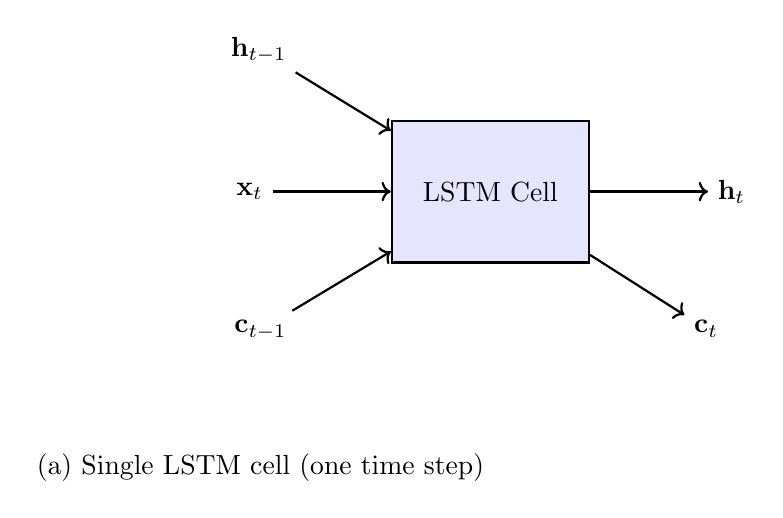
\begin{tikzpicture}[node distance=1.5cm and 1.5cm]
  \node[lstm] (cell) {LSTM Cell};
  \node[left=of cell] (xt) {$\mathbf{x}_t$};
  \node[above left=0.6cm and 1.2cm of cell] (htm1) {$\mathbf{h}_{t-1}$};
  \node[below left=0.6cm and 1.2cm of cell] (ctm1) {$\mathbf{c}_{t-1}$};
  \node[right=of cell] (ht) {$\mathbf{h}_t$};
  \node[below right=0.6cm and 1.2cm of cell] (ct) {$\mathbf{c}_t$};

  \draw[arrow] (xt) -- (cell);
  \draw[arrow] (htm1) -- (cell);
  \draw[arrow] (ctm1) -- (cell);
  \draw[arrow] (cell) -- (ht);
  \draw[arrow] (cell) -- (ct);

  \node[below=1.2cm of ctm1, align=center] {(a) Single LSTM cell (one time step)};
\end{tikzpicture}

\vspace{0.8cm}

% --- (b) LSTM Unrolled ---
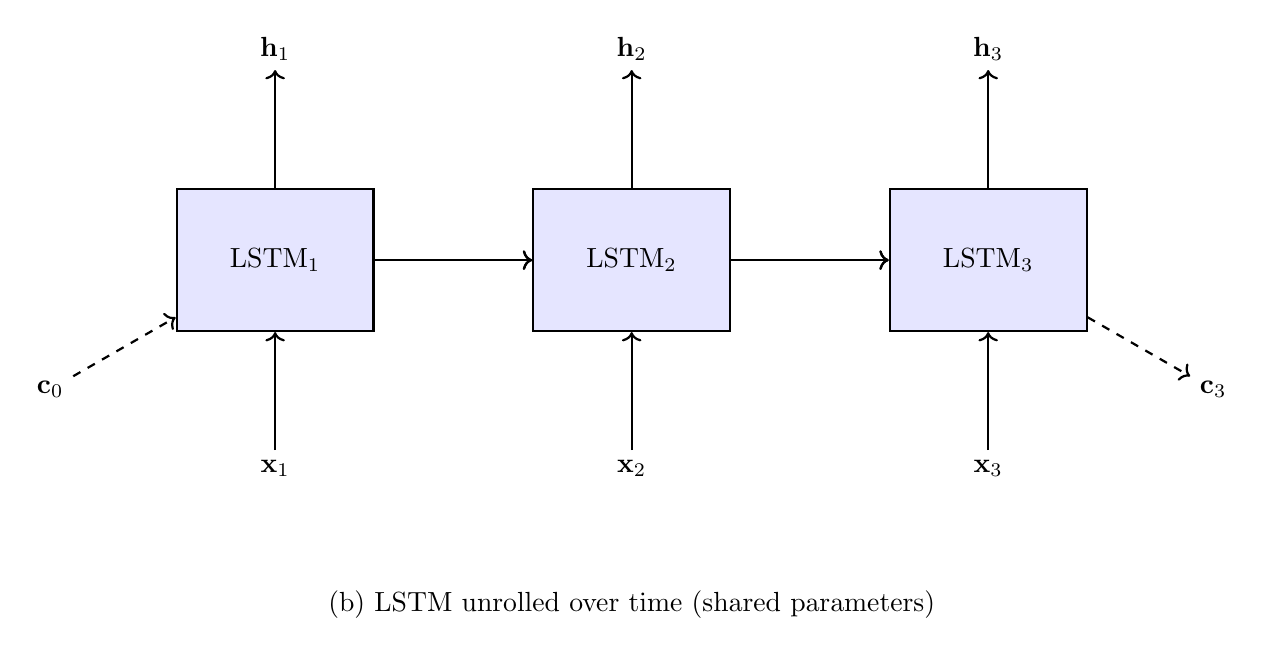
\begin{tikzpicture}[node distance=1.5cm and 2cm]
  % Cells
  \node[lstm] (cell1) {LSTM$_1$};
  \node[lstm, right=of cell1] (cell2) {LSTM$_2$};
  \node[lstm, right=of cell2] (cell3) {LSTM$_3$};

  % Inputs
  \node[below=of cell1] (x1) {$\mathbf{x}_1$};
  \node[below=of cell2] (x2) {$\mathbf{x}_2$};
  \node[below=of cell3] (x3) {$\mathbf{x}_3$};

  % Outputs
  \node[above=of cell1] (h1) {$\mathbf{h}_1$};
  \node[above=of cell2] (h2) {$\mathbf{h}_2$};
  \node[above=of cell3] (h3) {$\mathbf{h}_3$};

  % Connections
  \draw[arrow] (x1) -- (cell1);
  \draw[arrow] (x2) -- (cell2);
  \draw[arrow] (x3) -- (cell3);

  \draw[arrow] (cell1) -- (h1);
  \draw[arrow] (cell2) -- (h2);
  \draw[arrow] (cell3) -- (h3);

  \draw[arrow] (cell1) -- (cell2);
  \draw[arrow] (cell2) -- (cell3);

  % Cell state arrows
  \node[below left=0.5cm and 1.3cm of cell1] (c0) {$\mathbf{c}_0$};
  \node[below right=0.5cm and 1.3cm of cell3] (c3) {$\mathbf{c}_3$};

  \draw[arrow,dashed] (c0) -- (cell1);
  \draw[arrow,dashed] (cell1) -- (cell2);
  \draw[arrow,dashed] (cell2) -- (cell3);
  \draw[arrow,dashed] (cell3) -- (c3);

  \node[below=1.2cm of x2, align=center] {(b) LSTM unrolled over time (shared parameters)};
\end{tikzpicture}

\vspace{0.8cm}

% --- (c) Stacked LSTM ---
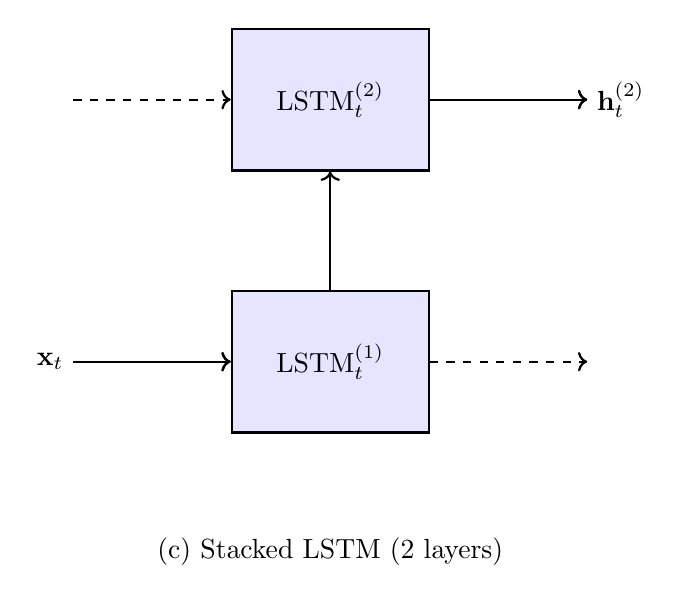
\begin{tikzpicture}[node distance=1.5cm and 2cm]
  % First layer
  \node[lstm] (cell1l1) {LSTM$_t^{(1)}$};
  \node[left=of cell1l1] (xt) {$\mathbf{x}_t$};
  \draw[arrow] (xt) -- (cell1l1);

  % Second layer
  \node[lstm, above=of cell1l1] (cell1l2) {LSTM$_t^{(2)}$};
  \draw[arrow] (cell1l1) -- (cell1l2);

  % Outputs
  \node[right=of cell1l2] (ht2) {$\mathbf{h}_t^{(2)}$};
  \draw[arrow] (cell1l2) -- (ht2);

  % Cell state arrows
  \node[left=of cell1l1] (c1in) {};
  \node[left=of cell1l2] (c2in) {};
  \node[right=of cell1l1] (c1out) {};
  \node[right=of cell1l2] (c2out) {};
  \draw[arrow,dashed] (c1in) -- (cell1l1);
  \draw[arrow,dashed] (cell1l1) -- (c1out);
  \draw[arrow,dashed] (c2in) -- (cell1l2);
  \draw[arrow,dashed] (cell1l2) -- (c2out);

  \node[below=1.2cm of cell1l1, align=center] {(c) Stacked LSTM (2 layers)};
\end{tikzpicture}
\caption{LSTM architectures. Solid arrows carry inputs and hidden states; dashed arrows carry the cell state $\mathbf{c}_t$. (a) One cell at one time step. (b) The same cell unrolled over three time steps; all three copies share one parameter set. (c) Two stacked layers at a single time step; the hidden state of layer 1 is the input to layer 2.}
\label{fig:lstm}
\end{figure}

\subsubsection*{Training Process}
Similar to RNNs, but gradients are better preserved:
\begin{enumerate}[label=\roman*)]
    \item Forward pass through LSTM cells, updating $\mathbf{h}_t$ and $\mathbf{c}_t$.
    \item Compute sequence loss (cross-entropy or MSE, as in Equations~\eqref{eq:xent} and \eqref{eq:mse}).
    \item Backpropagation Through Time with LSTM cell derivatives (mitigating vanishing gradient problem).
    \item Parameter update using optimizers.
\end{enumerate}

\subsubsection*{Step-by-Step Example}
Suppose:
\begin{itemize}
    \item Input: $x_1 = 1.0$
    \item Parameters: $W_f=W_i=W_c=W_o=1.0$, $U_f=U_i=U_c=U_o=0.5$
    \item Initial states: $h_0=0$, $c_0=0$
\end{itemize}

Step 1 (compute gates):
\begin{align*}
    f_1 &= \sigma(1.0) = 0.731, \\
    i_1 &= \sigma(1.0) = 0.731, \\
    \tilde{c}_1 &= \tanh(1.0) = 0.762.
\end{align*}

Step 2 (update cell state):
\begin{align*}
    c_1 &= 0.731 \cdot 0 + 0.731 \cdot 0.762 = 0.557.
\end{align*}

Step 3 (hidden state):
\begin{align*}
    o_1 &= \sigma(1.0) = 0.731, \\
    h_1 &= 0.731 \cdot \tanh(0.557) = 0.369.
\end{align*}

\noindent \textbf{Comment:} The cell state $c_1$ accumulates information additively, preserving memory over longer sequences.

\subsubsection*{Backpropagation Intuition}
From $c_t = f_t \odot c_{t-1} + i_t \odot \tilde{c}_t$, we have:
\begin{align}
    \frac{\partial c_t}{\partial c_{t-1}} = f_t.
\end{align}
If $f_t \approx 1$, gradients flow nearly unchanged across time, alleviating vanishing gradients. Contrast this with the RNN Jacobian $(1-h_t^2) W_{hh}$, which is squashed by the $\tanh$ derivative and rescaled by $W_{hh}$ at every step. The cell state is a highway along which information can travel long distances without being squashed by repeated $\tanh$ operations; each gate is a learned switch that decides whether information enters, stays on, or leaves that highway.

% ---------------------------------------------------------------------
\subsection{Stacked LSTM}
A stacked LSTM consists of multiple layers of LSTMs. The output of one layer becomes the input to the next, allowing the network to learn hierarchical features.

\subsubsection*{Equations}
For layer $\ell$ ($1 \leq \ell \leq L$):
\begin{align}
(h_t^{(\ell)}, c_t^{(\ell)}) = \mathrm{LSTM}^{(\ell)}(h_t^{(\ell-1)}, h_{t-1}^{(\ell)}, c_{t-1}^{(\ell)}),
\end{align}
with $h_t^{(0)} = x_t$. Written out for $L$ layers:
\[
\mathbf{h}_t^{(1)}, \mathbf{c}_t^{(1)} = \text{LSTM}^{(1)}(\mathbf{x}_t, \mathbf{h}_{t-1}^{(1)}, \mathbf{c}_{t-1}^{(1)}), \qquad
\mathbf{h}_t^{(2)}, \mathbf{c}_t^{(2)} = \text{LSTM}^{(2)}(\mathbf{h}_t^{(1)}, \mathbf{h}_{t-1}^{(2)}, \mathbf{c}_{t-1}^{(2)}), \qquad \dots
\]
\[
\mathbf{h}_t^{(L)}, \mathbf{c}_t^{(L)} = \text{LSTM}^{(L)}(\mathbf{h}_t^{(L-1)}, \mathbf{h}_{t-1}^{(L)}, \mathbf{c}_{t-1}^{(L)}).
\]
Final output is produced from the top layer $\mathbf{h}_t^{(L)}$.

\subsubsection*{Training Process}
\begin{enumerate}[label=\roman*)]
    \item Forward pass through all $L$ stacked layers.
    \item Compute sequence loss from top-layer outputs.
    \item Apply BPTT across both time steps and layers.
    \item Update parameters of all LSTM layers jointly.
\end{enumerate}
The loss remains the same (cross-entropy or MSE), applied at the top layer's output.

\subsubsection*{Step-by-Step Example}
Suppose the first layer outputs $h_1^{(1)} = 0.369$. This becomes the input to the second LSTM layer (with the same weights as the layer-1 toy example).

Step 1 (compute gates in layer 2):
\begin{align*}
    f_1^{(2)} &= \sigma(0.369) = 0.591, \\
    i_1^{(2)} &= 0.591, \\
    \tilde{c}_1^{(2)} &= \tanh(0.369) = 0.353.
\end{align*}

Step 2 (update cell in layer 2):
\begin{align*}
    c_1^{(2)} &= 0.591 \cdot 0 + 0.591 \cdot 0.353 = 0.209.
\end{align*}

Step 3 (compute hidden state in layer 2):
\begin{align*}
    o_1^{(2)} &= 0.591, \\
    h_1^{(2)} &= 0.591 \cdot \tanh(0.209) = 0.122.
\end{align*}

\noindent \textbf{Comment:} Layer 1 extracts features directly from the raw input. Layer 2 processes these features further, building hierarchical representations.

% ---------------------------------------------------------------------
\subsection{Parameter Sharing and Backpropagation in LSTMs}

\subsubsection*{Parameter Sharing Across Time}
An LSTM cell has learnable parameters for its gates:
\[
\theta = \{ W_f, W_i, W_c, W_o, U_f, U_i, U_c, U_o, b_f, b_i, b_c, b_o \}.
\]
When processing a sequence $\mathbf{x}_1, \mathbf{x}_2, \dots, \mathbf{x}_T$, the LSTM is \textit{unrolled} into $T$ cells (one per time step). Importantly, all $T$ cells share the same parameters $\theta$. This parameter sharing:
\begin{itemize}
    \item keeps the number of parameters independent of sequence length,
    \item allows the network to generalize patterns across different positions in the sequence.
\end{itemize}
Thus, while we draw multiple ``copies'' of the LSTM cell in diagrams (Figure~\ref{fig:lstm}b), mathematically there is only one set of weights applied repeatedly.

\subsubsection*{Parameter Sharing Across Layers}
In a \textit{stacked LSTM}, each layer has its own parameter set. For $L$ layers, we have
\[
\theta^{(1)}, \theta^{(2)}, \dots, \theta^{(L)},
\]
where parameters are shared across time within a layer but differ across layers.

\subsubsection*{Backpropagation Through Time (BPTT)}
During training, the loss is typically defined as the sum over time steps:
\[
\mathcal{L} = \sum_{t=1}^{T} \mathcal{L}_t.
\]
When computing gradients with respect to a shared parameter $W \in \theta$, we accumulate contributions from all time steps:
\[
\frac{\partial \mathcal{L}}{\partial W} = \sum_{t=1}^{T} \frac{\partial \mathcal{L}_t}{\partial W}.
\]
This ensures that weight updates reflect the influence of the entire sequence.

\noindent\textbf{Remarks.}
\begin{itemize}
    \item Across \textbf{time steps}: one parameter set is shared (no parameter explosion).
    \item Across \textbf{layers}: each layer has its own parameters.
    \item Backpropagation computes gradients through the unrolled network and accumulates them for the shared parameters.
\end{itemize}

% ---------------------------------------------------------------------
\subsection{Comparison and Discussion}
\begin{itemize}
    \item \textbf{RNN}: Simplest recurrent model. Struggles with long-term dependencies due to vanishing/exploding gradients.
    \item \textbf{Gated RNN (GRU)}: Introduces reset and update gates. More efficient than LSTM (fewer parameters) but less expressive in some tasks. Often performs competitively.
    \item \textbf{LSTM}: Introduces cell state with input, forget, and output gates. Best at capturing long-range dependencies. More parameters than GRU.
    \item \textbf{Stacked LSTM}: Adds depth to capture hierarchical and abstract sequence patterns.
\end{itemize}

\noindent \textbf{When to use:}
\begin{itemize}
    \item RNNs: For short sequences or when simplicity matters.
    \item GRUs: When training data is limited and efficiency is important.
    \item LSTMs: When modeling long-term dependencies is crucial.
    \item Stacked LSTMs: When tasks demand high capacity and abstraction.
\end{itemize}

\noindent \textbf{One more variant you will hear about.} A \emph{bidirectional} RNN or LSTM runs one recurrence forward and one backward over the sequence and concatenates the hidden states. It is useful when the whole sequence is available at training time (sequence labeling, the encoder of a translation system). It is \emph{not} usable for autoregressive generation, where only the past is available when each token is produced.

\subsection{Payoff (Key Takeaways)}
\begin{itemize}
    \item \textbf{RNN}: Direct recurrence. Simple, but struggles with long-term dependencies.
    \item \textbf{Gated RNN (GRU)}: Uses gates to mitigate vanishing gradients while being simpler than LSTMs.
    \item \textbf{LSTM}: Adds gates and a cell state to preserve information across long time spans.
    \item \textbf{Stacked LSTM}: Multiple layers enable deeper, more abstract sequence modeling.
\end{itemize}
You do not need to memorize the gate equations. The intuition you do need: each gate is a learned switch that decides whether information flows through, and the cell state is a highway that lets information (and gradients) travel long distances. Week 6 replaces the recurrence with self-attention; the autoregressive factorization of Topic 1 stays exactly the same.

\subsection*{Readings for Topic 2}
\begin{itemize}[nosep]\raggedright
\item D. Foster, \emph{Generative Deep Learning}, 2nd ed., Chapter 5, sections on RNN and LSTM architectures (companion notebook \texttt{05\_autoregressive/01\_lstm}).
\item S. Hochreiter and J. Schmidhuber, ``Long Short-Term Memory,'' \emph{Neural Computation} 9(8), 1997.
\item C. Olah, ``Understanding LSTM Networks,'' blog post, 2015.
\item K. Cho et al., ``Learning Phrase Representations using RNN Encoder-Decoder for Statistical Machine Translation,'' EMNLP 2014, arXiv:1406.1078 (the GRU paper).
\end{itemize}

\clearpage
% =====================================================================
\section{Topic 3: Sampling, Conditioning, and Sequence Quality}
% =====================================================================

\subsection{Plain-English summary}

Training an autoregressive model is the friendliest objective in deep learning: maximize the sum of next-token log-probabilities. Sampling from a trained model is where the engineering lives. The same model can produce dull, repetitive text (greedy decoding) or wildly incoherent text (high-temperature sampling) depending on which decoding strategy you pick. This topic walks through the standard decoding strategies, the conditioning patterns that let you steer the generator, the quality metrics you can compute, and the asymptotic cost of autoregressive sampling that nobody can engineer around.

\subsection{Decoding strategies: how to pick the next token}

At each step $i$ of generation the model returns a distribution $p_\theta(x_i \mid x_{<i})$ over possible next tokens (or pixels, or audio samples). You have to pick one. Write $z_k$ for the logit of token $k$, so that $p_\theta(x_i = k \mid x_{<i}) = \operatorname{softmax}(z)_k = e^{z_k} / \sum_j e^{z_j}$.

\paragraph{Greedy decoding.} Always pick the highest-probability token,
\begin{equation}
x_i = \argmax_k \; p_\theta(x_i = k \mid x_{<i}).
\end{equation}
Deterministic given the prefix and fast, but it produces repetitive, low-diversity output because the highest-probability path is often dominated by common short tokens. Almost never the right choice for open-ended generation.

\paragraph{Temperature sampling.} Sharpen or flatten the distribution before sampling:
\begin{equation}
p_T(x_i = k \mid x_{<i}) \;\propto\; p_\theta(x_i = k \mid x_{<i})^{1/T}
\quad\Longleftrightarrow\quad
p_T(x_i = k \mid x_{<i}) = \frac{e^{z_k / T}}{\sum_j e^{z_j / T}}, \qquad T > 0.
\label{eq:temperature}
\end{equation}
In plain language: $T = 1$ leaves the distribution unchanged; $T < 1$ sharpens it (closer to greedy; more deterministic, less diverse); $T > 1$ flattens it (more random, more diverse, more incoherent). As $T \to 0$ temperature sampling becomes greedy decoding; as $T \to \infty$ it becomes uniform over the vocabulary. For text, $T$ between 0.7 and 1.0 is the typical sweet spot; creative tasks push higher and factual completion lower. It is one of the few settings you tune by eye, and Foster's \texttt{01\_lstm} notebook implements it in a few lines.

\paragraph{Top-$k$ sampling.} Keep only the $k$ highest-probability tokens, renormalize, and sample from those. This cuts off the long tail of low-probability tokens that would otherwise occasionally produce nonsense. Typical $k$ for text: 20 to 50.

\paragraph{Top-$p$ (nucleus) sampling.} Holtzman et al.\ (2020) keep the smallest set $V_p$ of top tokens whose cumulative probability exceeds $p$,
\begin{equation}
V_p = \text{smallest } V \text{ (by descending probability) such that } \sum_{k \in V} p_\theta(x_i = k \mid x_{<i}) \ge p,
\end{equation}
then renormalize and sample within $V_p$. The nucleus adapts to the model's confidence: when the model is sure, only a few tokens clear the threshold; when it is uncertain, the set expands. Typical $p$: 0.9 to 0.95. Generally preferred over top-$k$ for natural-language generation.

\paragraph{Beam search.} Maintain $B$ candidate prefixes at each step, expand each by all possible next tokens, and keep the $B$ extended candidates with the highest total log-probability $\sum_{j \le i} \log p_\theta(x_j \mid x_{<j})$. Return the best complete sequence. Beam search is used where one best output matters more than diversity (machine translation, summarization, structured prediction). It is not used for open-ended generation because the approximately most-likely sequence is highly repetitive.

\subsection{Conditioning: steering what the model produces}

The vanilla autoregressive model has no knobs at inference: it samples $x_1 \sim p(x_1)$, then $x_2 \sim p(x_2 \mid x_1)$, and so on. To steer it, you add conditioning information $y$ that the model was trained to respect, so that every factor becomes $p_\theta(x_i \mid x_{<i}, y)$:
\begin{itemize}
\item \textbf{Prompt-based.} Prepend a token sequence $y$ to the input. The model continues from there. This is how language models work: there is no special ``prompt'' mechanism; the prompt is simply the start of the sequence.
\item \textbf{Class-conditional.} Train the model to take a class label as an additional input (concatenated to each time step's input, or used to initialize the hidden state). Foster's class-conditional PixelCNN is the example.
\item \textbf{Encoder context (seq2seq).} An encoder network compresses an input sequence into a context vector; the autoregressive decoder takes that as its initial state. This is the Sutskever et al.\ (2014) machine-translation setup, and the structure of every later encoder-decoder model.
\end{itemize}

\subsection{Quality metrics for autoregressive models}

\begin{itemize}
\item \textbf{Perplexity.} Exponentiated average negative log-likelihood per token,
\begin{equation}
\mathrm{PPL} = \exp\!\left(-\frac{1}{N} \sum_{i=1}^{N} \log p_\theta(x_i \mid x_{<i})\right).
\end{equation}
Lower is better. Native to autoregressive models because they have exact likelihood, and the standard metric for language models on held-out data. Use with caution: perplexity measures how well the model predicts your test set, not how good its samples look to a human. A model can have low perplexity and still generate incoherent text, because predicting the next token well (given a good prefix) and producing a good sequence (given your own imperfect prefix) are different tasks; this is the exposure-bias point from Topic 1.
\item \textbf{BLEU, ROUGE, METEOR.} Reference-based metrics for translation and summarization. Useful when a ground-truth output exists; useless for open-ended generation.
\item \textbf{FID (image autoregressive).} The same metric as for GANs in Week 3. Treat the autoregressive model as a sample source and compute FID against real images.
\item \textbf{Human evaluation.} Still the gold standard for open-ended generation. Quantitative metrics correlate imperfectly with human judgment.
\end{itemize}

\subsection{The unavoidable cost: $O(N)$ sampling}

To sample a length-$N$ sequence you must run the model $N$ times, once per token, and each step depends on all previous tokens, so the steps cannot be parallelized. This is intrinsic to the factorization \eqref{eq:chainrule}, not a software issue. Training does not have this problem: under teacher forcing all $N$ positions are scored in one pass.

For a 100-token text response on a modest LSTM the cost is invisible. For a $1024 \times 1024$ image on a PixelCNN (over one million pixels) it is brutal: hours of inference per image. The same problem affects WaveNet on raw audio, and it is the main reason diffusion models (Week 5), which denoise all positions in parallel, have largely displaced autoregressive image models for high-resolution work.

\subsection{Payoff}

A trained autoregressive model is only half of a generator; the decoding strategy is the other half. Temperature, top-$k$, nucleus, and beam search all read the same $p_\theta(x_i \mid x_{<i})$ and differ only in how they turn it into a choice. The Week 4 mini-lab asks you to run one Foster notebook with at least one decoding variation so that these knobs show up in your own samples.

\subsection*{Readings for Topic 3}
\begin{itemize}[nosep]\raggedright
\item D. Foster, \emph{Generative Deep Learning}, 2nd ed., Chapter 5, sections on generation and sampling.
\item A. Holtzman et al., ``The Curious Case of Neural Text Degeneration,'' ICLR 2020, arXiv:1904.09751 (Sections 1 to 4).
\item I. Sutskever, O. Vinyals, Q. V. Le, ``Sequence to Sequence Learning with Neural Networks,'' NeurIPS 2014, arXiv:1409.3215.
\item D. Bahdanau, K. Cho, Y. Bengio, ``Neural Machine Translation by Jointly Learning to Align and Translate,'' ICLR 2015, arXiv:1409.0473.
\end{itemize}

\clearpage
% =====================================================================
\section{Topic 4: Strengths and Limitations of Autoregressive Generation}
% =====================================================================

\subsection{Plain-English summary}

Autoregressive is the family behind the most widely deployed generative-AI systems today: every large language model, most code-completion systems, WaveNet-style audio synthesis, PixelCNN-style image generation, and protein-sequence design. It earned that position by being the easiest family to train with the most defensible probabilistic story. It also has hard limits: sampling is sequential and slow, the choice of ordering biases the model, and very long-range structure remained difficult until transformers solved a large part of it (Week 6). This topic puts autoregressive models side by side with VAEs (Week 2) and GANs (Week 3) so you can pick the right family for your project.

\subsection{Where autoregressive shines}
\begin{itemize}
\item \textbf{Exact likelihood.} No ELBO gap, no adversarial fixed point. The objective $\sum_i \log p_\theta(x_i \mid x_{<i})$ is well-conditioned, well-understood, and parallelizes across positions during training (even though sampling is sequential).
\item \textbf{Broad applicability.} Any data with a natural ordering works: text, code, audio, DNA, time series, and images via raster scan. The factorization $p(x) = \prod_i p(x_i \mid x_{<i})$ is universal in a way the latent-variable and adversarial setups are not.
\item \textbf{Strong tooling.} Hugging Face Transformers, PyTorch LSTMs, JAX models; every major framework has first-class autoregressive support and pre-trained checkpoints.
\item \textbf{Scales gracefully.} Bigger models, more data, and longer context windows keep improving performance (in a way GANs do not). The scaling-laws literature (Kaplan et al., 2020) is almost entirely about autoregressive models.
\item \textbf{Conditioning is easy.} Prepend the conditioning tokens, or start from a start-of-sequence token. The same mechanism handles everything.
\end{itemize}

\subsection{Where autoregressive struggles}
\begin{itemize}
\item \textbf{Sampling cost is $O(N)$ and not parallelizable across positions.} Every sample needs $N$ forward passes. For long sequences (high-resolution images, long-form audio) this is the bottleneck.
\item \textbf{The ordering choice biases the model.} A raster-scan PixelCNN sees the upper-left corner first and uses it to predict the rest; samples inherit a directional bias. There is no symmetric way to run autoregression on intrinsically unordered data.
\item \textbf{No bidirectional conditioning.} Modeling $p(x_i \mid x_{>i})$ (useful for infilling) needs a separate model or a non-autoregressive setup. BERT-style masked language modeling exists but is not a proper probabilistic model of the joint.
\item \textbf{Diversity and mode coverage depend on the sampler.} The same model gives excellent text at $T = 0.8$, nonsense at $T = 1.5$, and boring repetition at $T = 0$. Without a temperature knob you get one operating point.
\item \textbf{Long-range dependencies are hard for vanilla RNN/LSTM.} Even the LSTM struggles past a few hundred time steps. Transformers are the architectural fix.
\end{itemize}

\subsection{VAE versus GAN versus autoregressive}

Table~\ref{tab:families} extends the two-column comparison from Week 3 with a third column.

\begin{table}[htbp]
\centering
\small
\setlength{\tabcolsep}{5pt}
\renewcommand{\arraystretch}{1.15}
\begin{tabular}{@{}>{\raggedright\arraybackslash}p{2.9cm}>{\raggedright\arraybackslash}p{3.5cm}>{\raggedright\arraybackslash}p{3.5cm}>{\raggedright\arraybackslash}p{4.2cm}@{}}
\toprule
\textbf{Dimension} & \textbf{VAE} & \textbf{GAN} & \textbf{Autoregressive} \\
\midrule
Training objective & ELBO (lower bound on log-likelihood) & Minimax saddle point; no likelihood & Exact log-likelihood (sum of per-token terms) \\
Latent variable & Yes, with encoder $q_\phi(z \mid x)$ & Implicit (noise $z$ into generator) & None \\
Sample sharpness & Blurry (Gaussian decoder) & Sharp when training succeeds & Sharp; sequence quality varies with sampling strategy \\
Mode coverage & Broad (KL regularizer) & Can drop modes & Broad in principle; sampler-dependent \\
Training stability & Routine & Hard; many failure modes & Routine \\
Controllability & Latent arithmetic on $z$ & Conditional GAN, StyleGAN & Prompt-based conditioning \\
Likelihood evaluation & Lower bound only & None & Exact \\
Sampling cost & One forward pass & One forward pass & $O(N)$ sequential forward passes \\
Typical use cases & Representation learning, anomaly detection & High-quality image synthesis & Language, code, audio, DNA, anything with order \\
\bottomrule
\end{tabular}
\caption{The three generative-model families covered so far, compared on the same axes.}
\label{tab:families}
\end{table}

\subsection{Forward reference: transformers and diffusion}

Two developments since the LSTM era changed the field without changing the factorization of Topic 1.
\begin{itemize}
\item \textbf{Transformers (Week 6)} replaced recurrence with self-attention. Each factor $p_\theta(x_i \mid x_{<i})$ is still there; the function computing it becomes self-attention over the prefix instead of an unrolled recurrence. This made it possible to train much deeper and wider autoregressive models on much longer sequences. Every modern large language model is an autoregressive transformer.
\item \textbf{Diffusion (Week 5)} sidesteps the $O(N)$ sampling cost by training a model that denoises all positions in parallel over $T$ steps (typically 50 to 1000). Diffusion has largely displaced PixelCNN-style models for high-resolution images while leaving text and audio mostly to autoregressive transformers.
\end{itemize}

\subsection{Payoff}

You now have a working understanding of the third major family. When choosing a model for a project, the decisive questions are usually the ones in Table~\ref{tab:families}: Do you need a likelihood? Do you need a latent space? Is the data naturally ordered? Is $O(N)$ sampling acceptable? Autoregressive models answer ``yes, no, yes, it depends,'' and that profile explains both why they run the largest deployed systems and why diffusion took over high-resolution images.

\subsection*{Readings for Topic 4}
\begin{itemize}[nosep]\raggedright
\item D. Foster, \emph{Generative Deep Learning}, 2nd ed., Chapter 5, concluding sections.
\item J. Kaplan et al., ``Scaling Laws for Neural Language Models,'' 2020, arXiv:2001.08361.
\item A. Vaswani et al., ``Attention Is All You Need,'' NeurIPS 2017, arXiv:1706.03762.
\item T. Brown et al., ``Language Models are Few-Shot Learners,'' NeurIPS 2020, arXiv:2005.14165.
\end{itemize}

\end{document}
